% Title Page - No page numbering
\thispagestyle{empty}
\begin{center}
    \vspace*{2in}
    
    % Title
    \Huge\textbf{ScaloVit-EBM: Localized Energy-Based Anomaly Detection on Time–Frequency Scalograms}
    
    \vspace{1.0in}
    
    % Student Information
    \Large
    \textbf{Shosuke Asano} \\[0.3cm]
    \textbf{32201303}\\[0.3cm]
    FIT5128: Masters Thesis Final\\[0.3cm]
    Supervisor \textbf{Dr. Loo Junn Yong}\\[0.3cm]
    Co-Supervisor \textbf{Dr. Ting Chee Ming}\\[1cm]


    \vspace{0.5in}
    
    % Word Count
    \large
    \textbf{Word Count for Part 2 (Research Paper): 5556} words
    
    \vspace*{\fill}
    
    % Date
    \normalsize
    October 2025
    
\end{center}

\cleardoublepage
% Customize Contents header size and TOC font size
{
\renewcommand{\contentsname}{\huge Contents} % Adjust header size: \tiny, \scriptsize, \footnotesize, \small, \normalsize, \large, \Large, \LARGE, \huge, \Huge
\normalsize % Adjust TOC entries font size
\tableofcontents % This command generates the list based on \addcontentsline entries
}



\cleardoublepage
\pagenumbering{arabic} % Resume page numbering with Arabic numerals
\setcounter{page}{1} % Reset page counter if desired for this part (less common)
\phantomsection
\addcontentsline{toc}{section}{Part 1: Literature Review \& Proposal}
\label{part1}
\onecolumn
% Page numbers maintained for IEEE compliance
\vspace*{3in} % Add vertical space from the top
\begin{center}
    \Huge\textbf{Part 1: Literature Review} \\ % Use your actual title
    \vspace{0.5in}

\end{center}
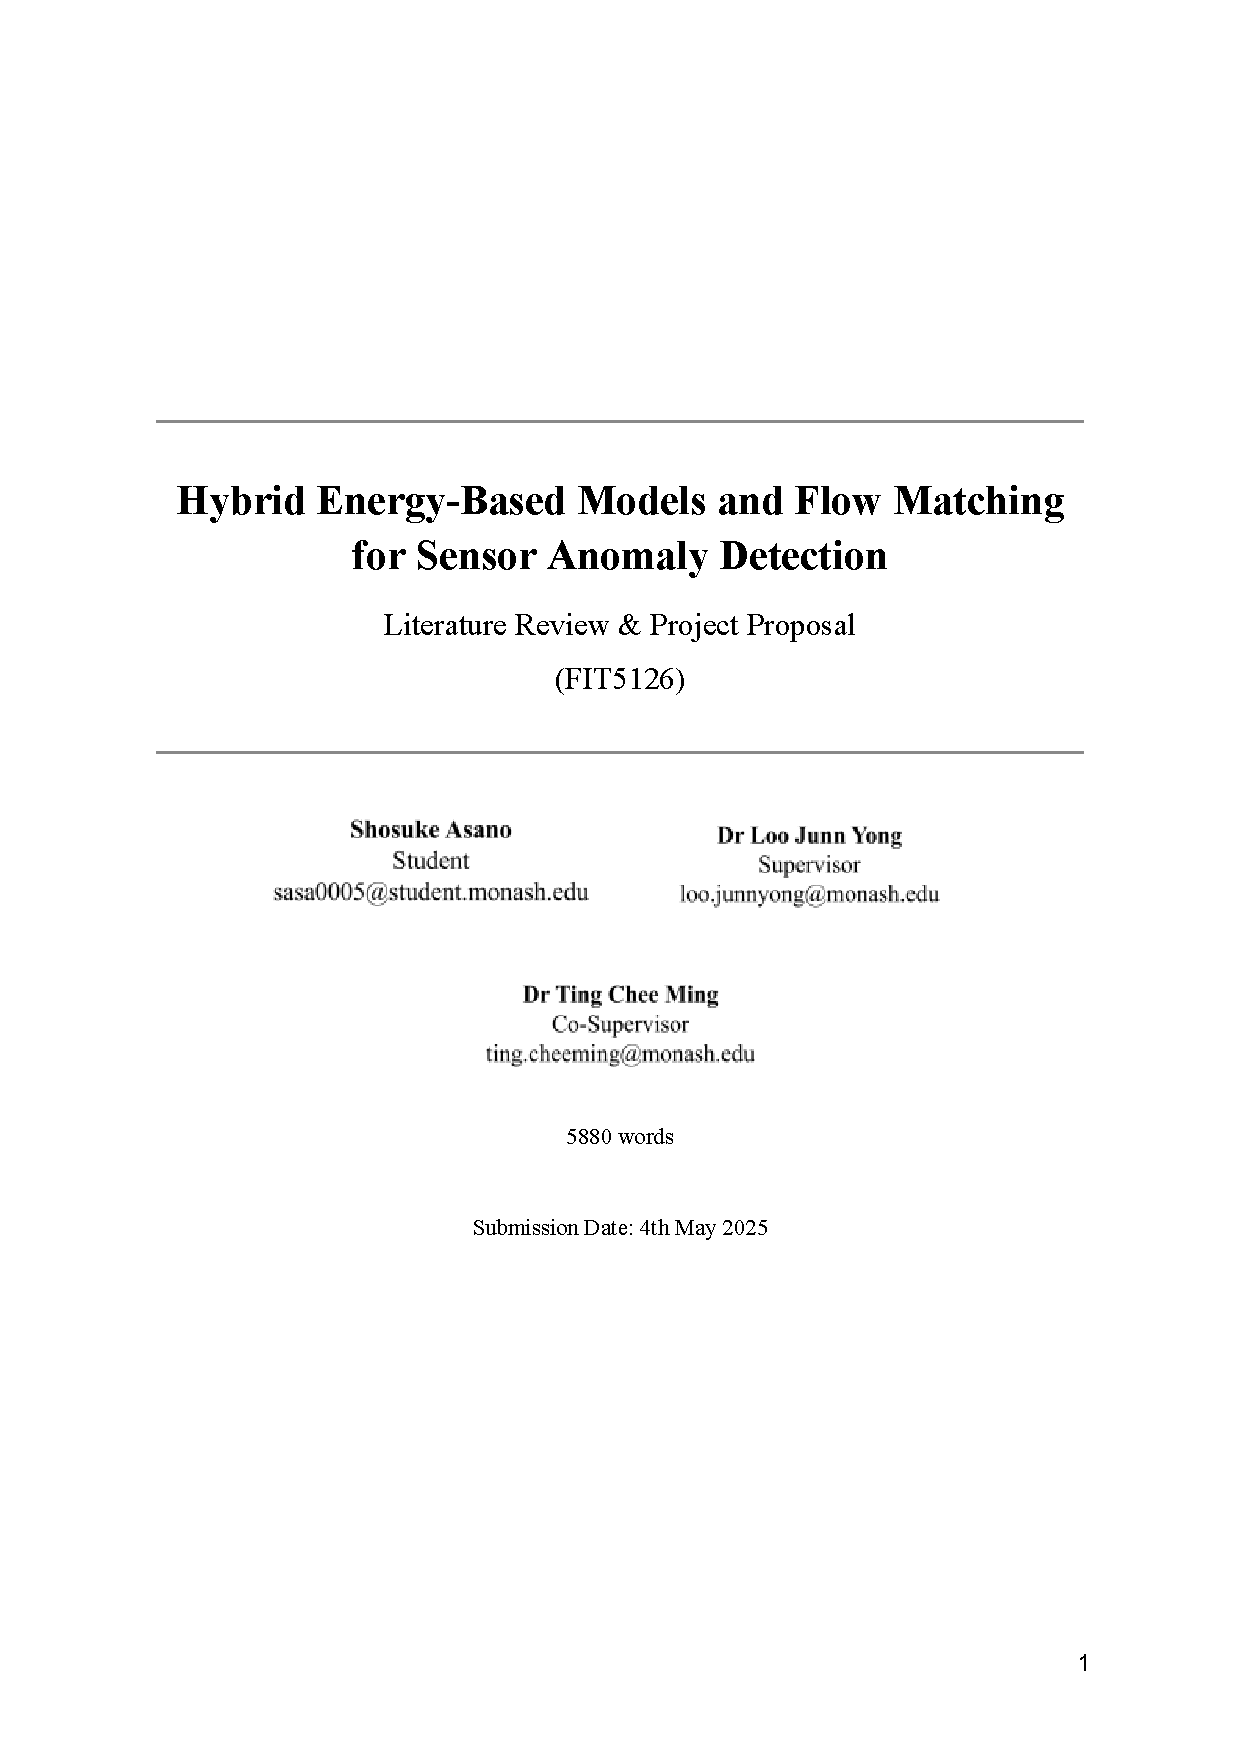
\includepdf[pages=-, link]{title/LitReviewProposal.pdf}
\cleardoublepage

\cleardoublepage
\phantomsection
\addcontentsline{toc}{section}{Part 2: Research Paper}
\label{part2}
% Page numbers maintained for IEEE compliance
\vspace*{3in} % Add vertical space from the top
\begin{center}
    \Huge\textbf{Part 2: Research Paper} \\ % Use your actual title
    \vspace{0.5in}

    % \Large (This section is included as reference by directly importing the PDF, so the page numbering for the section is independent of the main document.) \\
\end{center}
\cleardoublepage